\section{The internals of the compiler}

A compiler consists of several different parts: First of all, there's the source program which is the input to the compiler. The code is scanned so that a string of tokens can be created. These are then parsed forming an Abstract Syntax Tree (AST). A semantic analysis on the AST is performed, with the help of a symbol table, and the program is translated, optimized and finally the target code is generated. The process will be described to provide a little background knowledge of the compiler construction. 

Below is an illustration:

\begin{figure}[ht]
	\centering
		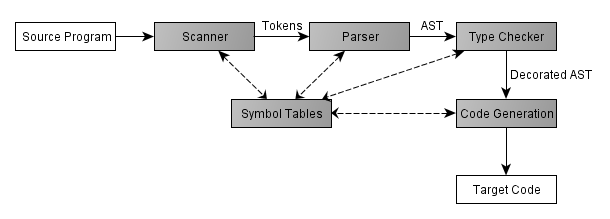
\includegraphics[scale = 0.5]{img/compiler.png}
	\caption{Compiler}
	\label{fig:compiler}
\end{figure}


\subsection{The Scanner}

The scanner is the part of the compiler responsible for transforming characters from the source program into a stream of tokens, i.e. the elementary symbols that define the language syntax, and the symbols that the parser can work with.
It is very important to have a formal definition of the tokens so that lexical rules are clearly stated and followed.
Tokens have two components: a type and a semantic value, the first indicating the token's membership in the terminal alphabet, the latter providing information about the token, if any is needed.
An example where the semantic value may not be needed is a terminal like "plus" in a simple calculator language. The terminal can only correspond to one token, namely the +. However for, say, an identifier it is important to have a semantic value to denote which identifier this is.
When the scanner tries to determine what kind of token is being scanned it will have a method that looks ahead, without removing the characters. Several algorithms for determining membership in the terminal alphabet can be employed, and often the scanner will also be instructed to skip certain parts of the code, like blanks and comment sections.
An example of the scanners token generation is shown below, with the line
\begin{lstlisting}
i a = 5
\end{lstlisting}

This generates 4 tokens: 
\begin{itemize}
\item A token of type "intdcl" (short for int declaration) with no need for a semantic value, as only the letter "i" corresponds to the type 
\item A token of type "id" with semantic value "a" 
\item A token of type "assign" with no need for a semantic value, as an assignment only corresponds to the "="
\item A token of type "inum" (short for integer numeral) with semantic value "5"
\end{itemize}

For a simple syntax an ad hoc scanner can be constructed to find the tokens, but for more complex syntaxes a scanner generator may be a time-saving choice.

\subsection{The Abstract Syntax Tree}
The AST is not an actual component of the compiler, but a data structure to help the Parser. It is a tree structure showing productions from the grammar. A production is the substitution of a variable with the terminal that rule can produce i.e. its production. The process of producing a sentence is shown in the AST with the root being the start variable, e.g. "Program", and the children being the terminals needed, e.g. "Decls" (declarations) or "Stmts" (statements). The leaves of the AST are the tokens input by the scanner.

\subsection{The Parser}

The parser is the part of the compiler that makes sure that the tokens generated by the scanner from the source code conform to the syntactical structure defined by the grammar of the language. The result is an AST. 

There are several ways to handle the parser problem, i.e. the problem of creating the parse tree from the token stream. Some parsers create the tree from the root to the leaves, called top-down or LL parsing, others create the tree from the leaves up, called bottom-up or LR parsing. 

Top-down parsing works by creating a procedure for each non-terminal. If, for example, there is a rule "Program $\rightarrow$ Dcls | Stmts \$" the parser determines if this is a case of a declaration or a statement by looking ahead at tokens until it knows which one it is. The term LL stands for Left to right, Leftmost derivation, which signifies that the parser reads the stream from left to right and makes leftmost derivations.

An LL(k)-parser works by looking ahead at the next k tokens to decide which production to use. Generally as low a value of k as possible is preferable as the look-ahead takes time. 

Bottom-up works by reading the stream until it has a set of tokens that fits a rule in the grammar. The LR stands for Left to right, Rightmost derivations, i.e. the parser reads the stream from left to right and makes rightmost derivations.

An LR(k)-parser reads tokens until only one production rule applies. For each node in the AST it then checks if the node and its children can generate a parent node.

The top-down approach to parsing is easy and quickly implemented and therefore often used, however they cannot parse grammars where tokens share common prefixes, or grammars with left-recursive rules, and thus LR-parsers are considered stronger parsers.

\subsection{Type Checking}

The semantic analysis creates what is called a decorated AST. What it does is check what is called the static semantics of each node. This means that each node is meaningful and legal with regards to type etc. for the source language. If it is, the node is decorated with  type information. Should an error be discovered, an error message is sent out. 

The definition of a type varies, but common for all languages is the notion that types are a certain set of values, and some operations on these values, e.g. a Boolean variable has only the values true and false every time the program runs.

\subsection{The Symbol Table}

The symbol table is a central table accessible from all compiler phases which contains information that is associated with identifiers. When an identifier is declared, its information is stored in the symbol table, so that the next time it is used it can be retrieved from the table. This is used in type checking.

\subsection{The Optimizer}

Optimization of the code means analysing and transforming the IR code, so that it does the same, but is more efficient thus speeding up the target code. This is a quite complex phase, which, especially if a high level of optimization is chosen, will take longer than if no optimization is chosen.

\subsection{The Code Generator}
This is where the target code is generated from the decorated AST. This phase need detailed knowledge the target machine, e.g. register allocation, code scheduling and so on. This phase is often coded by hand instead of using a tool, and a good code generator requires many special cases to be considered.